\chapter[SPC]{Statistical Process Control- SPC}
\label{sec:spc}

Statistical process control (SPC), \aka \emph{change detection}, or \emph{novelty detection}, deals with the quantitative analysis of a ``process'', which may be a production line, a service, or any other repeated operation.\marginnote{Change Detection}
As such, SPC may be found in the Analyze, Improve, and Control stages of the DMAIC cycle.
The purpose of the SPC, in the terms coined by Shewart, is to seperate the variability in the process into \emph{assignable} causes of variation and \emph{chance} causes of variation.\marginnote{Causes of variation}
Assignable are also known as \emph{special} causes, or simply \emph{signal}.
Chance causes are also known as \emph{common} causes of variation, or \emph{haphazard} variability, or simply \emph{noise}.
 
A process is said to be in \emph{statistical control} if all its variation is attributable to chance causes.
If this is not the case, we call it \emph{out of control} and we will seek the assignable causes, so that we may reduce variability by removing them.
All the statistical tools of chapters \ref{sec:exploratory} and \ref{sec:inference} may be called upon for this endeavour but in this chapter we focus on one particular such tool- the \emph{control chart}.
We start with the \emph{Shewart control chart}, in which each value is charted using different data, from different periods. \marginnote{Shewart Chart}



\begin{extra}[A mathematically rigorous treatment of SPC]
The contents of this chapter is mostly derived from \cite{montgomery_introduction_2007}. 
For a more mathematically rigorous treatment of the topic see \cite{basseville_detection_1993}.
For an \R oriented exposition of the topic, see \cite{qiu_introduction_2013}.
\end{extra}

\section{A soft start. The \barxChart}

We demonstrate the concepts and utility of control charts with the simplest, yet most popular of them all, the \barxChart. 
The chart borrows its name from the fact that it is essentially a visualization of the time evolution of the average ($\bar{x}$) of the CTQ. 
The chart is also augmented with visual aids that help in determining if the process is \emph{in control}, i.e., if it is consistent with its own history. 

\begin{remark}[Control Charts and Capability Analysis]
Control charts have no information on the specifications of the process, merely on its own history.
Process capability analysis may, however, benefit from the ideas of control charts, as we explain in Chapter~\ref{sec:advanced_capability_analysis}.
\end{remark}


An illustration of a \barxChart is given in Figure~\ref{fig:bar_x_chart}. 
The ingredients of this chart are the centerline, lower and upper control limits (LCL, UCL), and $\bar{x}$ evolving in time. 
If at each period $t=1,\dots,\tau$ we compute the average of $n$ samples, we denote $$\bar{x}_t:=1/n \sum_{i=1}^n x_{it}.$$

\begin{figure}[ht]
\centering
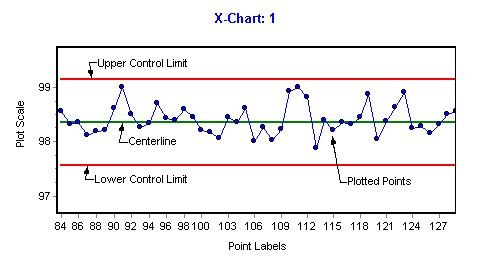
\includegraphics[height=0.3\textheight]{art/X-chartExample}
\caption[\barxChart]{\barxChart. \newline \url{https://mvpprograms.com/help/P-mvpstats/spc/WhatAreControlCharts}}
\label{fig:bar_x_chart}
\end{figure}



Figure~\ref{fig:bar_x_chart} makes it evident \barxChart requires us to make several design decisions.
A standard design decision is setting the center line as the grand average of the process: 
\begin{align}
\label{eq:centerline}
	\hat{\mu}_0=1/\tau \sum_{t=1}^\tau \bar{x}_t,
\end{align}
where $\mu_0$ denotes the in-control mean of the process. 
Notation originates from treating the in-control process as a null hypothesis, as it should be thought of.


If it is unclear to you, how may we compute the grand average of a process that is still evolving and has not finished, you are right! We thus introduce the idea of \emph{Phase I} and \emph{Phase II}. \marginnote{Phase I/II}
Initially we assume the process it out of control, we identify and remove assignable causes of variation, until we are left with a ``well-behaved'' subset of data points, we believe to be in-control. We call this Phase I, and we use it to initialize required quantities such as the centre line. 
Eq.(\ref{eq:centerline}) thus implies that in Phase I we were left with $\tau$ samples assumingly in statistical control.
After the chart has been calibrated, and major assignable sources of variability removed, we can finally start monitoring the process, known as Phase II.



Other design decisions to be made are:
\begin{enumerate}
\item UCL and LCL (Do not confuse with USL and LSL!).
\item Sample size in each sample ($n$).
\item The within period sampling scheme, known as \emph{rational groupings}.
\item The between-period sampling scheme, notably the \emph{frequency of samples}. 
\item Other stopping rules.
\end{enumerate}
These design decisions ultimately govern the error rates of the chart, which in turn, incur financial costs. 
For now we will restrict attention to type I/II error rates, until Section~\ref{sec:economical_considerations} where we consider these choices as economical optimization problems.

For ease of exposition, control chart design is demonstrated for the \barxChart, but equally applies to other control charts, presented in Section~\ref{sec:other_control_charts}.
We start by a type I error rate analysis. 
Denote $\alpha_t$ the false alarm probability at period $t$.
How do our design choices affect $\alpha_t$?
\begin{align}
	\alpha_t &:= 1-P_{H_0}(\bar{x}_t \in [UCL,LCL]) \\
	&= 2 P_{H_0}(\bar{x}_t<UCL) \\
	&= 2 P_{H_0}(Z<\frac{UCL-\mu}{\sigma_{\bar{x}}}) \\
	&= 2 P_{H_0}(Z < -\arm) \\
	&= 2 \Phi(-k)
\end{align}
The above follows from assuming that $UCL:=\mu_0 + \arm \sigmabar, LCL:= \mu_0 - \arm \sigmabar$, $\x_{it}\sim \gauss{\mu,\sigma^2}$, and denoting $\sigmabar:= \frac{\sigma}{\sqrt{n}}$.
A typical design choice is $\arm=3$, known as \emph{3-sigma control limits}, implying a false alarm rate of $\alpha_t=0.0027$.\marginnote{3-Sigma Control Limits}
Since we assumed the process is fixed over time, then so is $\alpha_t$ and we can simply write $\alpha_t=\alpha$.

\begin{remark}[3-Sigma Control Limits vs. 3-Sigma Capability]
Do not confuse these two similar ideas.
3-Sigma Control Limits is a statement on the false alarm rate of a process with respect to its own \textbf{history}.
3-Sigma Capability is a statement on the non-compliance rate of a process with respect to its \textbf{specification}.
\end{remark}


A power analysis for our design choices follows the same lines.
Denote by $H_1$ the out-of-control distribution,  $\beta_t$ the type-II error rate, and $\pi_t=1-\beta_t$ the power, at period $t$.
We then have
\begin{align}
	\pi_t &:= 1-P_{H_1}(\bar{x}_t \in [UCL,LCL])
\end{align}
and the rest follow from the distribution of $\bar{x}$ when the process is out of control.
Since the out-of-control shift is (asumingly) stable, we can again omit the time index and write $\pi=\pi_t$.
Assuming the out-of-control process is a shift of magnitude $k \sigma$, i.e.: $\x \sim_{H_1} \gauss{\mu_1,\sigma^2}; \mu_1=\mu_0+ k \sigma$, we plot in Figure~\ref{fig:power_function}, the detection power of a 3-sigma \barxChart, as a function of $k$. 
This is known in the statistical literature as a \emph{power function}, and in the engineering literature as the \emph{true positive rate} operator characteristic (TPR-OR).\marginnote{Operator Characteristic}


\begin{figure}[h]
\centering
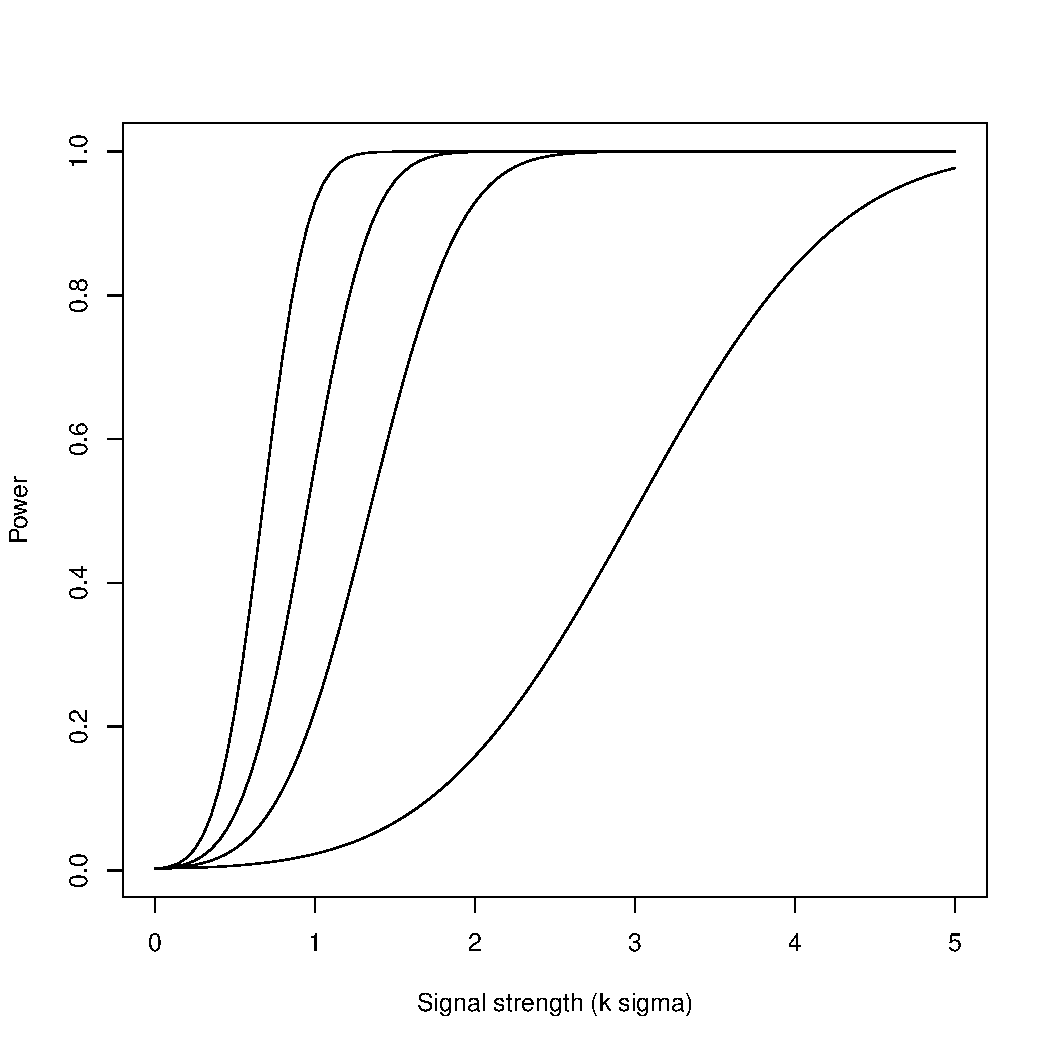
\includegraphics[height=0.3\textheight]{art/power_function.pdf}
\caption[Power Function]{Power function of the 3-sigma \barxChart with $n=5,10,20$ and $\mu_1=\mu_0 + k \sigma$.}
\label{fig:power_function}
\end{figure}

\begin{extra}[Operator Characteristics]
Many operator characteristics have been proposed to study the performance of control charts, statistical tests, or binary classifiers in general.
You may be already familiar with some, such as the ROC-curve. 
The curious reader is referred to \cite{wikipedia_receiver_2015} for more information.
\end{extra}


An important related quantity is the \emph{average run length} (ARL), which is the expected number of periods between two crossings of control limits, i.e., the expected periods between alarms. \marginnote{ARL}
We denote by $ARL_0$ the ARL when the process is under statistical control, and $ARL_1$ otherwise\footnote{Note that it is implied that the process has a \emph{stable} distribution, even though it is out if control.}. 
For Shewart charts, where $\bar{x}_t$ are typically statistically independent, then clearly the number of periods until a crossing is geometrically distributed. Using the expectation of a geometric random variable we can conclude that 
\begin{align}
	ARL_0=1/\alpha \label{eq:arl_0}, \\
	ARL_1=1/\pi \label{eq:arl_1}.
\end{align}
Clearly we can convert to time units by multiplying the ARL by the duration of sampling interval.
This is known as the \emph{average time to signal} (ATS).\marginnote{ATS}
It is quite common to design a control chart so that it achieves a particular $ATS_0$.

\begin{remark}[ARLs more important than type-I errors]
In the case of Shewart charts, there is a simple mapping between ARL and type I error rates.
This need not be the case for general control charts. 
Since type I errors are certain, if the process runs long enough, then it is actually the ARL the design parameter of importance, and not the type-I erro.
\end{remark}


Now assume that we are unhappy with some control chart. 
It simply makes too many false alarms, or takes too long to detect loss of statistical control.
What can we do about it?
Well, this is exactly the same question as when increasing the power or lowering the type I error of a statistical hypothesis test. This is obviously no coincidence, since control charts are nothing but a statistical test!
Here are some action courses:
\begin{enumerate}
\item Increase $\arm$. This is the same as shrinking the rejection region: 
it will decrease the false alarm rate, at the cost of power.
\item Increase $n$. Brilliant! Statistically, there is nothing to lose. It may, however, cost time and money.
\item Increase the sampling frequency. Brilliant again! Nothing to lose, except time and money...
\item Change the sampling scheme within period. We elaborate on this in Section~\ref{sec:rational_grouping}.
\item Add other stopping rules: 
this acts just like growing the rejection region. It will increase power, at the cost of type I error. We elaborate in Section~\ref{sec:stopping_rules}.
\item Pool together more time points or more CTQs. We elaborate on this in sections \ref{sec:running_windows} and  \ref{sec:multivariate}, respectively. 
\end{enumerate}






\subsection{Control Limits and the Alarm Rate}
As previously discussed, $\arm$ governs the tradeoff between type I and type II errors, or sensitivity versus specificity.
It is very common to set $\arm=3$. 
For a Normally distributed CTQ, this implies $2,700$ false alarms per million periods. 
This also implies an $ARL_0$ of $1/\alpha \approx 370$ periods.
We may obviously, discard this $\arm=3$ convention, and directly set UCL and LCL so they guarantee some desirable false alarm rate. 

If normality of $\bar{x}_t$ can be assumed, then one may estimate $\sigma$ from phase I, and set LCL and UCL by finding the $\arm$ that solves $2\Phi(-\arm)=\alpha$.
If normality cannot be assumed, there are many ways to go about. Here are some options:
\begin{enumerate}
\item Increase $n$: even if $\x_it$ is non normal, for large enough $n$, then $\bar{x}_t$ will be via the central limit theorem (CLT).
\item Use empirical quantiles: If phase I was returned enough data, then we may estimate $\x_{\alpha/2}$ and $\x_{1-\alpha/2}$ using the empirical quantiles of phase I. The false alarm rate will be $\alpha$ since $P(\x \not \in [\x_{\alpha/2},\x_{1-\alpha/2}])=\alpha$.
\item If some other distribution can be assumed then we may compute the false alarm rate of particular limits either analytically, or computationally (by simulation).
\end{enumerate}




\subsection{Rational Groupings}
\label{sec:rational_grouping}
Recall that at each period we compute the average of $n$ samples. 
How should we draw these samples? All at the same time from the same machine?
At different times from the same machine?
Many configurations are possible, and the correct approach depends on the type of out-of-control behaviour one seeks. 
\emph{Rational groupings} merely reminds us to sample ``rationally'' in each period. 
Quoting \cite{montgomery_introduction_2007}'s words of caution:
\begin{quotation}
\dots we can often make any process appear to be in statistical control just by stretching out the interval between observations in the sample.
\end{quotation}






\subsection{Other Stopping Rules}
\label{sec:stopping_rules}

The assumption that we may only create alarms if $\bar{x}$ exceeds some control limits is needlessly restrictive.
A first relaxation is by allowing multiple regions.
It is quite common to define \emph{warning limits} which only call for inspection, and \emph{action limits}. Each may have its own alarm rate.
We may even change the sapling scheme if limits are breached. Increasing the sampling rate once the warning limits have been breached is known as \emph{adaptive sampling}, or \emph{variable sampling}.\marginnote{Adaptive Sampling}



Another approach is to define multiple sets of stopping rules.
Here is an example:
\begin{enumerate}
\item One or more points outside of the 3-sigma control limits.
\item Two of three consecutive points outside the 2-sigma warning limits but still inside the 3-sigma control limits.
\item Four of five consecutive points beyond the 1-sigma limits.
\item A run of 8 consecutive points on one side of the center line.
\end{enumerate}
The above set of rules is known as the Western Electric Rules, \aka\, the \emph{WECO} rules.\marginnote{WECO}
Augmenting the set of rules is the same as increasing a rejection region. It adds more sensitivity, at the cost of false alarms. If the rules are properly selected, the gain in sensitivity is worth the increase in false alarms.

As a quick exercise, we may compute $\alpha$  for $m$ independent rules, each with $\alpha^*$ type I error itself:
\begin{align}
	\alpha=1-(1-\alpha^*)^m.
\end{align}
Having 4 rules, like WECO, each at $\alpha^*0.0027$ implies that we actually have $\alpha=0.01$.

\begin{extra}[Stopping Rules]
There are many sets of stopping rules. 
These include WECO, Nelson, AIAG, Juran, Hughes, Duncan, Gitlow, Westgard, and more. 
See \url{http://www.quinn-curtis.com/spcnamedrulesets.htm} for a quick introduction.
\end{extra}


% TODO: Yoav and Kling paper.




\section{Pooling Information Over Periods}
\label{sec:running_windows}

Assume an out-of-control process is simply a mild shift of the controlled-process.
This shift may be hard to detect in Shewart chart, especially if $n$ is not too large (as seen in Figure~\ref{fig:power_function}).  
If the shift persists, we may gain power, i.e., sensitivity, by pooling several periods together. 
We now present several ways to pool information from history. These are typically applied in Phase II, where out-of-control processes are expected to have only mild shifts, and not major ones as in Phase I. 

\begin{remark}[No longer Shewart]
The name \emph{Shewart control chart} is reserved to charts plotting one period at a time. 
When several periods are pooled together, we will no longer call this  ``Shewart''.
\end{remark}

\begin{remark}[One observation at a time]
The following charts have a continuous flavour. As such, it is both favourable, and common, to compute them using one observation at a time, and not by grouping, as is typically for Shewart charts. 
\end{remark}



\subsection{Run Test Chart}
[TODO]




\subsection{Moving Average Chart- MA}
One way to pool information from different periods is by a \emph{moving average}.
\begin{definition}[Moving Average- MA]
The moving average at period $t$ is defined as
\begin{align}
	M_t:= \frac{x_t+\dots+x_{t-w+1}}{w}
\end{align}
\end{definition}
Assuming $x_t \sim \gauss{\mu_0, \sigma_x^2}$ then clearly 
\begin{align}
	M_t \sim \gauss{\mu_0, \frac{\sigma_x^2}{w}}.
\end{align}

The control limits on $M_t$ are typically
\begin{align}
	UCL &:= \mu_0 + 3 \sigma_{M_t}= \mu_0 + 3 \, \frac{\sigma_x}{\sqrt{w}} \\
	UCL &:= \mu_0 - 3 \sigma_{M_t}= \mu_0 - 3 \, \frac{\sigma_x}{\sqrt{w}}.
\end{align}
The fallout rate of this criterion is trivially $\alpha=0.0027$. 
The $ARL_0$ is no longer simple to compute. 
This is because the pooling of periods has compromised independence between periods, and Eqs.(\ref{eq:arl_0},\ref{eq:arl_1}) are no longer valid. 
Do not despair as the ARL may still be computed. 
You can always use simulation to compute it, or try using the \rcode{spc} \R package.


%\begin{algorithm}[$ARL_0$ simulation for MA Control Chart]
%\caption{$ARL_0$ simulation for MA Control Chart}
%\begin{algorithmic}
%\For {$\bootstrap \in 1,\dots,\bootstraps$}
%	\State $\sample^\bootstrap \gets$ $n$ randomly selected observations, with replacement, from the original data.
%	\State $\sample^\bootstrap_\rank \gets$ $\rank$ randomly selected variables from $\sample^\bootstrap$.
%    \State $\estim{\hyp}^{\bootstrap} \gets$ a tree learned with  $\sample^\bootstrap_\rank$.
%\EndFor
%\State \Return the the average prediction for $x$ over $\estim{\hyp}^{\bootstrap}$ .
%\end{algorithmic}
%\end{algorithm}


We are free to choose the magnitude of $w$. 
If $w$ is too small, there is no real pooling from history. At the limit, where $w=1$, we are back to the classical Shewart chart. 
If $w$ is too large, then each new observation has very small importance, and it may take a long time to detect a shift.
Which is the right intermediate value of $w$, is left for you to decide.






\subsection{Exponentially Weighted Moving Average Chart- EWMA}
The moving average gives all observations the same importance. 
We want to change this, giving more importance to new observations so that we may capture drifts quickly when they occur. 
The \emph{Exponentially Weighted Moving Average} (EWMA), \aka the \emph{geometric moving average} (GMA), does just that. \marginnote{GMA}
\begin{definition}[Exponentially Weighted Moving Average- EWMA]
\begin{align}
	z_t &:= \lambda x_t + (1-\lambda) z_{t-1}
\end{align}
\end{definition}
By recursive substitution, we have 
\begin{align}
	z_t &:= \lambda \sum_{j=0}^{t-1} (1-\lambda)^j x_{t-j} + (1-\lambda)^t z_0,
\end{align}
and 
\begin{align}
\label{eq:ewma_variance}
	z_t &\sim \gauss{\mu_0,	\sigma^2_{z_t} }, \\
	\sigma^2_{z_t} &= \sigma^2_x \left( \frac{\lambda}{2-\lambda} \right)(1-(1-\lambda)^{2t}).
\end{align}
Eq.(\ref{eq:ewma_variance}) may be used to construct control limits for EWMA:
It is however, more economic to observe that for large $\lambda$ and $t$: $(1-(1-\lambda)^{2t}) \approx 1$ so that we may use 
\begin{align}
\begin{split}
\label{eq:ewma_variance_approximate}
	UCL &:= \mu_0 + 3 \sigma_{z_t} \approx \mu_0 + \arm \, \sqrt{\sigma^2_x\left( \frac{\lambda}{2-\lambda} \right)},  \\
	UCL &:= \mu_0 - 3 \sigma_{z_t} \approx \mu_0 - \arm \, \sqrt{\sigma^2_x\left( \frac{\lambda}{2-\lambda} \right)},
\end{split}
\end{align}
with $\arm=3$ being the typical choice.
By now, you should immediately know what is the fallout rate of these limits.
By now, you should also know that because of the dependence between $z_t$'s, computing the ARL is not as simple as for Shewart charts. The \rcode{xewma.arl()} \R function, in package \rcode{spc}, permits doing so easily. 
Its output for various $\lambda$ and $\arm$ is illustrated in Figure~\ref{fig:arl_0_ewma}.

\begin{figure}[h]
\centering
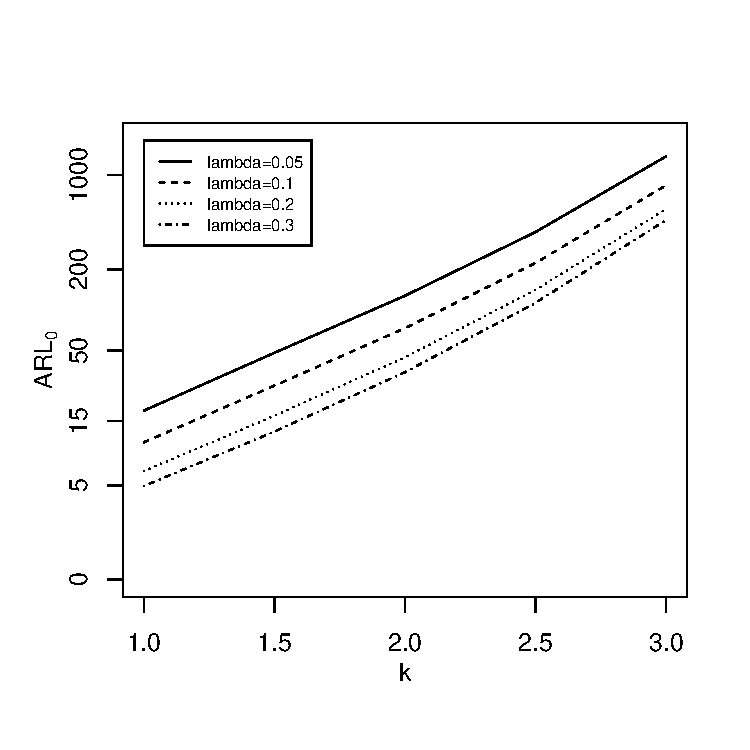
\includegraphics[height=0.3\textheight]{art/fig53}
\caption[$ARL_0$ for EWMA]{$ARL_0$ for EWMA. \newline Code from \url{http://users.phhp.ufl.edu/pqiu/research/book/spc/r-codes/fig53.r}}
\label{fig:arl_0_ewma}
\end{figure}

Note that if we do not opt for the approximation in Eq.(\ref{eq:ewma_variance_approximate}), and use the exact Eq.(\ref{eq:ewma_variance}) then the alarm limits change over time. 


In the MA chart, we used the choice of $w$ to balance between quick response (small $w$) and sensitivity (large $w$).
EWMA has no window-width parameter, since it looks into all of history. On the other hand, we can control it by choosing $\lambda$. 
Large $\lambda$ gives more importance to the present. At the limit, $\lambda=1$, EWMA collapses to a standard Shewart chart.







\subsection{Filtered Derivative Chart}
[TODO]


\subsection{CUSUM Chart}
The \emph{cumulative sum} chart is similar to the EWMA in that it pools information from the history. 
The CUSUM simply sums all past deviations from the centre line.
If the process is in control, deviation will cancel each other, and their sum will vary around $0$. 
If the process is ot of control, a drift will appear. 
The statistic to be plotted is 
\begin{align}
	C_t:= \sum_{j=0}^{t}(x_j-\mu_0)=C_{t-1}+ (x_t-\mu_0)
\end{align} 
Observing that when under control then $C_t \sim \gauss{\mu_0, t \sigma_x^2}$, we could set 
\begin{align}
\label{eq:cusum_simple_limits}
\begin{split}
	UCL &:= \mu_0 + 3 \sigma_{C_t}= \mu_0 + \arm \, \sqrt{t \sigma_x^2},  \\
	UCL &:= \mu_0 - 3 \sigma_{C_t}= \mu_0 - \arm \, \sqrt{t \sigma_x^2}.
\end{split}
\end{align}
You may encounter these limits in your favourite software (\rcode{qcc} package in \R?), but it less often discussed in the literature. 
This is because CUSUMs were introduced by \cite{page_continuous_1954}, which offered different control limits. 
\cite{montgomery_introduction_2007} adopts \citeauthor{page_continuous_1954}'s view and presents limits in two forms: the \emph{decision interval} (DI) form, \aka the \emph{tabular} form, and the graphical form known as a \emph{V-mask}.
These two control limits are equivalent. Before we present them, we try to offer some intuition for the difference between the limits in Eq.(\ref{eq:cusum_simple_limits}) and those of \cite{page_continuous_1954}.

The fundamental difference between the control limits of \cite{page_continuous_1954}, and the ones presented until now, is that \citeauthor{page_continuous_1954} designed limits for the particular history of each process, while the limits until now, including Eq.(\ref{eq:cusum_simple_limits}) do not adapt to the particular history of the process.
As such, \citeauthor{page_continuous_1954}'s control limits are said to be \emph{adaptive}.\marginnote{Adaptive Contol Limits}

[TODO: explain V-mask and tabular]





\subsection{Shiryaev-Roberts Procedure}
[TODO]

%\begin{extra}[Wald's Sequential Likelihood Ration Test- SPRT]
%[TODO]
%\end{extra}




\subsection{Combined Shewart and Running Window Charts}






\begin{extra}[Local Methods]
% scan statistic
% sliding window
% search light
% Anomaly detection active learning
\end{extra}








\section[Multivariate]{Multivariate Control Charts}
\label{sec:multivariate}
% Wishart
% Srivastava Du
% PCA
% Higher criticism

\begin{example}[Intensive Care Unit]
\label{eg:intensive}
Consider an intensive care unit. 
The CTQs are the patient's blood pressure, temperature, etc.
We want to sound an alarm if the patient's condition deteriorates. 
Clearly, we can apply previous the univariate methodology above. 
It is possible, that the deterioration is mild, so that it is not picked up by any CTQ individually (low power), but could have been noticed were we to aggregate signal from all CTQs. 
\end{example}
This is the concern of the current section. 

\subsection{Mass Univariate Control}
\label{sec:mass_univariate}

A first natural approach is to raise an alarm when \textbf{any} of the processes exceeds its respective control limits.
For $m$ independent processes, with false alarm rate $\alpha$ each, then the joint false alarm rate is 
\begin{align}
	\alpha^* = 1-(1-\alpha)^m.
\end{align}
Clearly we could set $\alpha=1-\sqrt[m]{1-\alpha^*}$, so that the joint false alarm rate is under control, but we would not be enjoying the added sensitivity of pooling many CTQs together. 



\subsection{Hotteling's \tsq}
Hotteling's \tsq statistic is a generalization of the t-test.
To see this we write the t-statistic in the following weird form:
\begin{align}
	t(x)=(\bar{x}_t-\mu_0) (s^2_t(x))^{-1} (\bar{x}_t-\mu_0).
\end{align}
This notation readily extends to the multivariate case. 
For $p$ CTQs, then $\bar{x}_t$ and $\mu_0$ are $p$-length vectors, and $s^2_t(x)$ is replaced with the $p \times p$ matrix $\hat{\Sigma}_t(x)$.
\begin{definition}[Hotteling's \tsq]
\begin{align}
\label{eq:hotteling}
	T^2_t := n (\bar{x}_t-\hat{\mu}_0)' \hat{\Sigma}_t^{-1} (\bar{x}_t-\hat{\mu}_0).
\end{align}
\end{definition}
To derive the control limits, we will be assuming that $\x_{it}$ is $p$-variate Gaussian distributed, $\gauss{\mu_0, \Sigma_{p \times p}}$. 
We need to be very clear, however, on how $\mu_0$ and $\Sigma_t^{-1}$ are estimated. 
We thus consider the following scenario:
\begin{enumerate}
\item \tsq is computed at Phase II with a single observation at a time ($n=1$)
\item $\mu_0,\hat{\Sigma}_t^{-1}$ were estimated from $m$ observations in Phase I.
\end{enumerate}
Eq.(\ref{eq:hotteling}) thus yields 
\begin{align}
	T^2_t := (x_t-\hat{\mu}_0)' \hat{\Sigma}_t^{-1} (x_t-\hat{\mu}_0).
\end{align}
and 
\begin{align}
	T^2_t \sim F_{p,m-p} \frac{p(m-1)(m+1)}{m(m-p)} \overset{m \to \infty}{\rightsquigarrow }\chi^2_p.
\end{align}
We can thus construct the control limit for this scenario:
\begin{align}
	UCL:= F_{1-\alpha,p,m-p} \frac{p(m-1)(m+1)}{m(m-p)} \approx \chi^2_{1-\alpha,p}.
\end{align}
Note that the \tsq statistic is \emph{non directional}: it will increase in the presence of both positive and negative drift. 

We may consider the distribution of \tsq under many configurations: where $\mu_0,\hat{\Sigma}_t^{-1}$ are estimated at Phase II, where we take $n$ observation in each period, etc. 
For our current purposes, we will use the fact that if $n \gg p$, or $m \gg p$, then 
\begin{align}
	T^2_t  \rightsquigarrow \chi^2_p,
\end{align}
and thus
\begin{align}
	UCL \approx \chi^2_{1-\alpha,p}.
\end{align}

\begin{extra}
For exact results and references on the various scenarios described, we refer the reader to \cite[Ch.7]{qiu_introduction_2013}.
\end{extra}

Since the above limits have an (approximate) type-I error rate of $\alpha$, and the periods are typically independent, then we can readily apply Eq.(\ref{eq:arl_0}) to compute $ARL_0$.



\subsection{Extra Info- Other Pooling Statistics}
Hotteling's \tsq implicitly targets a weak signal on many coordinates. 
In the signal detection literature, this is known as a \emph{dense} signal.
In our intensive care unit example (Example~\ref{eg:intensive}), it may be the case the a patient's deterioration is mildly manifested in many CTQs. It may however, be the case, that deterioration is manifested in a small subset of CTQs.
This is further emphasized in Example~\ref{eg:cyber}.

\begin{example}[Cyber Monitoring System]
\label{eg:cyber}
Consider a server farm. All servers dump their status into logs. These include CPU loads, temperature, network I/O, etc.
The administrator is worried about an imminent attack, and it thus parsing the logs for CTQs, and inspecting the on-line status on his dashboard.
He knows that the cyber-attacker is no amateur, so that if any fingerprint is left in the logs, it will be very subtle. 
\end{example}

The intensive care example, and the cyber security example, motivate our search for a statistic, that unlike Hotteling's \tsq, is sensitive to \emph{sparse} signals. \marginnote{Sparse Signal}
I.e., a signal that is manifested in very few of the $p$ CTQs.
For this purpose, we merely offer several candidate multivariate statistics, with references where appropriate.
\begin{description}
\item [Max pooling] Where we control the process using the $\max$ over CTQs. Useful when we expect signal in a handful of CTQs.
\item [Higher Criticism] Where pooling is performed using the Higher Criticism statistic. Appropriate for an intermediate \emph{rare-weak} sparsity pattern. See details in \citep{jin_cosmological_2005}.
\item [Skewness Statistic] Where pooling is performed using the empirical third moment. Appropriate for an intermediate sparsity pattern. See details in \citep{jin_cosmological_2005}.
\end{description}







\section{Economical Design of Control Charts}
\label{sec:economical_considerations}

Up until now, our design of control charts was driven by type-I error rates, and ARLs. Economical consideration were merely implied.
In this section, economical consideration take the driver's seat. 
We present a toy model, to demonstrate the economical optimization of design parameters in a \barxChart. 
Before beginning, a few remarks are in order. 

\begin{remark}[Economical Design of Control Charts]
\noindent
\begin{enumerate}
\item According to \cite{montgomery_introduction_2007} 
\begin{quote}
Saniga and Shirland (1977) and Chiu and Wetherill (1975) report that very few practitioners have implemented economic models for the design of control charts.
\end{quote}
Hmmmm.. Have things changed since 1977?
\item A comprehensive theoretical analysis of the optimization of a quality control system may be found in \cite{girshick_bayes_1952}. Again, \cite{montgomery_introduction_2007} is skeptic:
\begin{quote}
The optimal control rules are difficult to derive, as they depend on the solution to
complex integral equations. Consequently, the model’s use in practice has been very
limited.
\end{quote}
\end{enumerate}
\end{remark}

In light of the above skepticism, and following the lines of \cite{duncan_economic_1956}, we aim at the modest goal of an economical optimal \barxChart. 
Our target function is optimizing the expected income per hour, with respect to the design parameters:
\begin{align}
\label{eq:optimal_design}
	\max_{n,\arm,h}\set{\expect{C/T}}
\end{align}
where $C$ is the income between two productions halts, i.e., a \emph{cycle};
$T$ is the cycle duration;
$n$ is the number of samples per period;
$\arm$ governs the control limits via $UCL:= \mu_0+ \arm \sigma_{\bar{x}}= \mu_0+ \arm \sigma_x / \sqrt{n}$;
$h$ is the time interval between sample periods. 

We now need to establish how $\expect{C/T}$ is related to $n,\arm,h$. Here is our set of assumptions and notation:
\begin{enumerate}
\item When in control (IC), production is centred on $\mu_0$, assumed known. 
\item When out of control (OC), $\mu_1=\mu_0 \pm \delta \sigma_x$. 
\item When OC, production may proceed (!). 
\item Search and repair costs are not part of $C$.
\item OCs occur as a Poisson process, with rate $\lambda$ events per hour. The expected time from a sampling to an OC events is thus 
\begin{align}
	\tau := \frac{1-(1+ \lambda h) e^{-\lambda h}}{\lambda(1-e^{-\lambda h})}
\end{align} 
\item The power to detect an OC is 
\begin{align}
	\pi:= \Phi(-\arm-\delta/\sqrt{n})+ (1-\Phi(\arm-\delta/\sqrt{n}))
\end{align}
\item The false alarm rate
\begin{align}
	\alpha:= 2 \Phi(-\arm)
\end{align}
\item Because of the Poisson process assumption,  $\expect{C/T}=\expect{C}/\expect{T}$. 
\item The expected cycle length:
\begin{align}
	\expect{T}= \frac{1}{\lambda}+ \frac{h}{\pi}- \tau  + D
\end{align}
where $\frac{1}{\lambda}$ is time IC;
$\frac{h}{\pi}- \tau$ is the time the process is OC until detection;
$D$ is a fixed time to identify the assignable cause. 
\item The expected income per cycle
\begin{align*}
	\expect{C}= V_0 \frac{1}{\lambda} + 
	V_1 \left(\frac{h}{\pi}- \tau  + D  \right) - 
	a_3 -
	\frac{a'_3 e^{-\lambda h}}{1-e^{-\lambda h}} -
	(a_1+a_2n)\frac{\expect{T}}{h}
\end{align*}
where $V_0$ is the net income per cycle when IC;
$V_1$ is the net income when OC;
$(a_1+a_2n)$ is the fixed and variable cost of taking a sample;
$a_3$ is the cost of finding an assignable cause;
$a'_3$ is the cost of investigating a false alarm.
\end{enumerate}

Given all the above, we may now plug Eq.(\ref{eq:optimal_design}) into our favourite numerical solver to find the optimal $h,\arm,n$.



\section{Shewart Charts With Other Test Statistics}

We have been focusing on the \barxChart for ease of exposition. There are, however, many cases where the mean is not an appropriate test statistic.
Examples include:
\begin{enumerate}
\item A discrete CTQ, where only the number of non-compliances can be counted. 
\item Where the departure from statistical control is not only a shift in $\mu$.
\end{enumerate}

The following charts are designed for those cases. 
Practically all of the ideas presented for the \barxChart may be adapted to these other test statistics after appropriate adaptations. 
The reader is referred to \cite{montgomery_introduction_2007} for the details. 

\label{sec:other_control_charts}
\subsection{$R$ Chart}
Where $\bar{x}$ is replaced by the range. 
Sensitive to variability changes. 
Popularized by its ease of implementation, in the pre-PC age. 
\subsection{$s$ Chart}
Where $\bar{x}$ is replaced by $s$. 
Sensitive to variability changes. 
Usually more sensitive than the range.
\subsection{$s^2$ Chart}
Like the $s$ chart, only in variance-scale.
\subsection{$p$ and $np$ Chart}
Where $\bar{x}$ is replaced by the proportion ($p$), or number ($np$), of non-conforming units.
Appropriate for attributes, i.e., discrete QTCs.
\subsection{$c$ Chart}
Like a $np$ chart, but where the number of nonconforming units is replaced with the total number of nonconformances, allowing multiple defects per unit. 
\subsection{$u$ Chart}
Like the $c$ chart, but allowing a variable number of units per sample (varying $n$).
\subsection{Regression Control Chart}
In a \emph{regression control chart}, the test statistic can be a regression coefficient. 
When compounded with multivariate charts, a regression control chart may accommodate several regression  coefficient, or the residuals. 




\section[Extensions]{Extensions of Control Charts}
We have been discussing the simplest of \barxChart chart, for ease of exposition.
Several immediate extensions are possible.
The reader is referred to \cite{montgomery_introduction_2007} for details.
\begin{description}

\item [One sided charts] Just like hypothesis testing, where we may consider non-directional or directional hypotheses, we may consider directional control chart. 
Obviously the control limits and the test statistic may need appropriate updates.

\item [Autocorrelation and time series models] The assumption of independence between sampling periods may be relaxed, by adopting a quantitative or qualitative model for temporal dependence.

\item [Running Window Versions] The ideas of pooling information over periods with a moving averages, EWMA, and CUSUM may be extended to all type of Shewart charts. 

\item [Multiple Charts] When inspecting a process, rarely does one inspect a single chart at a time. A typical dashboard would include several charts running in parallel, as depicted in Figure~\ref{fig:dashboard}.

\end{description}



\subsection{Cuescore Charts}
[TODO]



